\setchapterpreamble[u]{\margintoc}
\glsresetall % reset glossary
\chapter{Optimizing the layout of the modules in space}
\todo{tables always small}
Introduction

\section{Optimize the modules' layout using a modified DMO algorithm}
The goal is to treat the problem of contemporanely optimizing the modules' layout and topology of a modular structure. the major scientific challange is that the layout optimization of the modules in the structure subdomains is a discrete problem, where we can't have interediate results at the end of the optimization. As we want to use a gradient descent algorithm \sidecite{sigmund_usefulness_2011} for this reason we need to find a method to transform a discrete problem into a continuous one. 

\subsection{Definition of the subdomains cross-sectional areas}
inspired by the work of stegmann and lund on the \gls{dmo} algorithm \sidecite{stegmann_discrete_2005}, we decided here to define the subdomains variables (so the variables of the structure) as a weighted sum of the modules variables. In the case of a ground structure discretized using Nsub subdomains and Nt different modules, we define then the cross sectional areas of the subdomain j as:
\begin{equation}
    \vect{a}^j = \sum_{t=1}^{N_T} w_t^j \bar{\vect{a}}_t 
\end{equation}
where $\bar{\vect{a}}_t $ represent the vector of cross sectional areas of the t module and $\vect{w}^j$ is the vector of weight relatives to the j subdomain, defined as $ \vect{w}^j \in \mathbb{R}^t\,|\,w_j^t \in [0,1]$.

An exemple of a cantilever beam with Nsub = 8 and Nt = 2 is given in \figref{fig:06_weighted_sum}, where we see how the modfication of the weight values $\vect{w}$ influences the structure topology.

\begin{figure*}
    \centering
    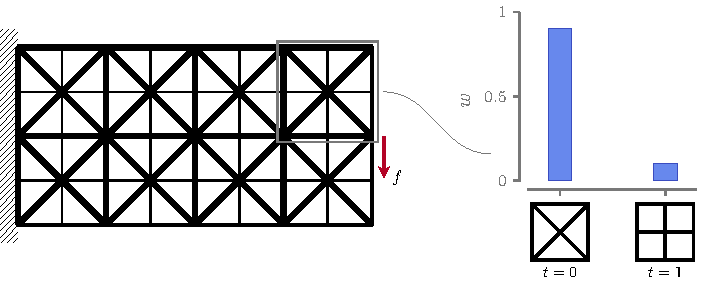
\includegraphics{figures/06_DMO/00_weight_dmo/weight_dmo.pdf}
    \caption{}
    \label{fig:06_weighted_sum}
\end{figure*}

\subsection{Variables penalization schemes}
The limit of the presented approach lies in the fact that at convergence, the weight of every subdomains mus be all zero but one to one . This is because intermediate weights would represent a mix of different topologies that would not have mechanical sense and that would prove to be impossible to manufacture. For that reason we implement here an interpolation scheme that penalize intermediate densities. We use here \gls{ramp} \sidecite{stolpe_alternative_2001} and not the more used SImp interpolation scheme as RAMP because the derivative it is never infinite nor 0 at zero density.

We define the design variable $\alpha$ responsable of the module choiche inside of the subdomain j. its relationship with the weight $w$ is the following: 
\begin{equation}
    w_t^j = \frac{\alpha_t^j}{1+p(1-\alpha_t^j)}    
\end{equation}
where $p\in \mathbb{R}^+$ is a parameter used to control the steepness of the RAMP interpolation. Additionally, inspired by the works of \sidecite{hvejsel_material_2011}, we put up a multi-phase versions of the RAMP interpolation where we simultaneously penalize mechanical properties and we artificailly icrease the volume of modules with intermediate densities. To do that we define an additional RAMP parameter, this thime always negative $q\in \mathbb{R}^-$ that is used to evaluated the increased weights associated with the evaluation of the volume $V$.
\begin{equation}
    V = \sum_{j=1}^{N_{\text{sub}}}\vect{\bar{\ell}}^T\tilde{\vect{a}}^j,
\end{equation}
where $\tilde{a}$ is defined as following:
\begin{equation}
    \tilde{\vect{a}}^j = \sum_{t=1}^{N_T} \tilde{w}_t^j \bar{\vect{a}}_t, 
\end{equation}
and $\tilde{w}$
\begin{equation}
    \tilde{w}_t^j = \frac{\alpha_t^j}{1+q(1-\alpha_t^j)}.    
\end{equation}
So for every design variable alpha, we associate two different weights (w and tilde w) that are used to evaluate the mechanical properties and the structure volume, respectively (see \figref{fig:06_ramp}).

\begin{figure}
    \centering
    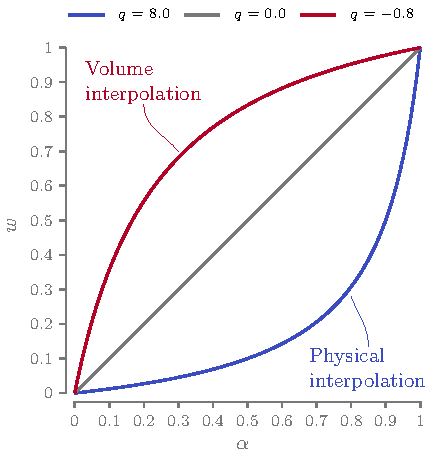
\includegraphics{figures/06_DMO/00_ramp/ramp.pdf}
    \caption{}
    \label{fig:06_ramp}
\end{figure}

\subsection{The optimization formulation and resolution algorithm}
The objective function of the optimization process is the volume minimization of the modular structure. 
The members of the structure are subject to multiple mechanical constraints, namely stress, topological buckling, minimum slenderness, and compatibility constraints. Formulation $\mathbb{M}_1$ is stated in terms of modules' cross-sectional area $\bar{\vect{a}}$, module selection variables $\vect{\alpha}$, member forces $\vect{q}$ and nodal displacements $\vect{U}$ as follows:
\begin{equation}
    \begin{aligned}
    \min_{\bar{\vect{a}}, \vect{\alpha}, \bm{q}, \bm{U}}   && V &= \sum_{j=1}^{N_{\text{sub}}}\vect{\bar{\ell}}^T\tilde{\vect{a}}^j && \textrm{(Volume minimization)}\\
    \textrm{s.t.}   && \bm{B}\bm{q} &= \bm{f} && \textrm{(Force equilibrium)}\\
                    && \bm{q} &= \frac{\bm{a}\bm{E}}{\bm{\ell}}\bm{b}^T\bm{U} && \textrm{(Compatibility constraints)} \\
                    && \bm{q} &\geq -\frac{\bm{s}\bm{a}^2}{\bm{\ell^2}} && \textrm{(Euler buckling constraints)} \\
                    && -\sigma_C\bm{a} &\leq \bm{q} \leq \sigma_T\bm{a} && \textrm{(Stress constraints)} \\
                    && \bar{\vect{a}}_{t,r}&\geq \bar{a}_{t,r=1} && r \in \mathcal{C}_{l,r}(\bar{\vect{a}}_t),\, \forall t \\
                    && 0 &\leq \bar{\vect{a}} \leq \frac{4 \pi \bar{\vect{\ell}}^2}{\lambda_{\text{max}}} && \textrm{(Slenderness limit)} \\
                    && \sum_{t=1}^{N_T} \alpha_t^j &\leq 1, \; \forall j && \textrm{(One selected module max.)} \\
    \end{aligned}
    \tag{$\mathbb{M}_1$}
    \label{eq:06_optim_complete}
\end{equation}

This formulation builds on the classic DMO approach, adding multiple mechanical constraints, operating on a ground structure, but most importantly we are not only selecting the best module for every subdomain changing the value of $\alpha$, but we are also optimizing the also the modules topology, and all of this at the same time. Tihis is more difficoult. The qvqntqges of this formulation are essentially the fact that wa are dealing with discrete problem and solving it using continuous design variables and a gradient based optimizer. However, we increase considerably the size of the problem, as we are adding numerous additional design variables $\alpha$ that scales with the number of subdomains and the number of modules.

The design variable alpha are constrained by a set of constraint that constraint the maximum sum of weights of a j submodule to one. it is important to note that we are treating this constraint as a disequality constraint and not an equality, and for this reason we give the optimizer the ability to put al the weights to zero and remove the subdomain from the steucture.
\begin{equation}
    \sum_{t=1}^{N_T} \alpha_t^j \leq 1, \; \forall j 
\end{equation}

Problem \eqrefnotext{eq:06_optim_complete} is solved using a modified version of the proposed two step solving algorithm, in wich we solve a relaxed problem without compatibility constraints kinematic compatibility constraints are omitted. We call this relaxed Problem $\mathbb{M}_2$. this time, as the problem is nonlinear due to the alpha design variables, we solve it without linearizing the buckling constraints.  here is the formulation of the first subproblem:

\begin{equation}
    \begin{aligned}
    \min_{\bar{\vect{a}}, \vect{\alpha}, \bm{q}}   && V &= \sum_{j=1}^{N_{\text{sub}}}\vect{\bar{\ell}}^T\tilde{\vect{a}}^j && \textrm{(Volume minimization)}\\
    \textrm{s.t.}   && \bm{B}\bm{q} &= \bm{f} && \textrm{(Force equilibrium)}\\
                    && \bm{q} &\geq -\frac{\bm{s}\bm{a}^2}{\bm{\ell^2}} && \textrm{(Euler buckling constraints)} \\
                    && -\sigma_C\bm{a} &\leq \bm{q} \leq \sigma_T\bm{a} && \textrm{(Stress constraints)} \\
                    && 0 &\leq \bar{\vect{a}} \leq \frac{4 \pi \bar{\vect{\ell}}^2}{\lambda_{\text{max}}} && \textrm{(Slenderness limit)} \\
                    && \sum_{t=1}^{N_T} \alpha_t^j &\leq 1, \; \forall j && \textrm{(One selected module max.)} \\
    \end{aligned}
    \tag{$\mathbb{M}_2$}
    \label{eq:06_optim_relax}
\end{equation}

We fix the module layout on the structure and we evaluate the corresponding mapping matrix H. Then the compatibility constraints are added again
we solve it fixing the submodules topology and using the VL formulation already used in \dots
we have no alpha anymore
\marginnote{Formulation ${\mathbb{M}}_\text{1}$ permits to optimize modular structures with fixed module layout. It is stated in terms of modular cross-sectional areas $\bar{\vect{a}}$, member forces $\vect{q}$ and nodal displacements $\vect{U}$ as follows:
\begin{equation*}
    \begin{aligned}
    \min_{\bar{\vect{a}}, \vect{q}, \vect{U}}   && V &= \vect{\ell}^{T}\vect{a}\\
    \textrm{s.t.}  && \vect{a} &= \sum_{t=1}^{N_\text{T}} \vect{h}_t\otimes\bar{\vect{a}}_t \\ 
    && \matr{B}\vect{q} &= \vect{f} && \\
    && \vect{q} &= \frac{\vect{a}E}{\vect{\ell}}\vect{b}^T\vect{U} &&  \\
    && \vect{q} &\geq -\frac{s\vect{a}^2}{\vect{\ell}^{*2}} &&  \\
    && -\sigma_c\vect{a} &\leq \vect{q} \leq \sigma_t\vect{a} &&  \\
    && \bar{\vect{a}}_{t,r}&\geq \bar{a}_{t,r=1}\\
    && 0 &\leq \bar{\vect{a}} \leq \frac{4 \pi \bar{\vect{\ell}}^2}{\lambda_{\text{max}}}, \\
    \end{aligned}
\end{equation*}
}
\subsection{Optimization initialization: a clustering algorithm to identify similarly behaving subdomains}
we are not only changing the weights but also the modules topology.  the layout is dependent on the module topology and vice versa. so we give a slighltly influenced departure point x0. In this work we decided to infuence the weight distribuition as follows:
\begin{equation}
    \alpha_{t,\text{it}=0}^j=
    \begin{cases}
        \frac{1}{N_\text{T}} \cdot 1.1  & \text{if the $j$-th subdomain has the  $t$-th module selected,}\\
        \frac{N_\text{T}-1.1}{N_\text{T}(N_\text{T}-1)} & \text{otherwise.} \\
    \end{cases}  
\end{equation}

\begin{figure*}
    \centering
    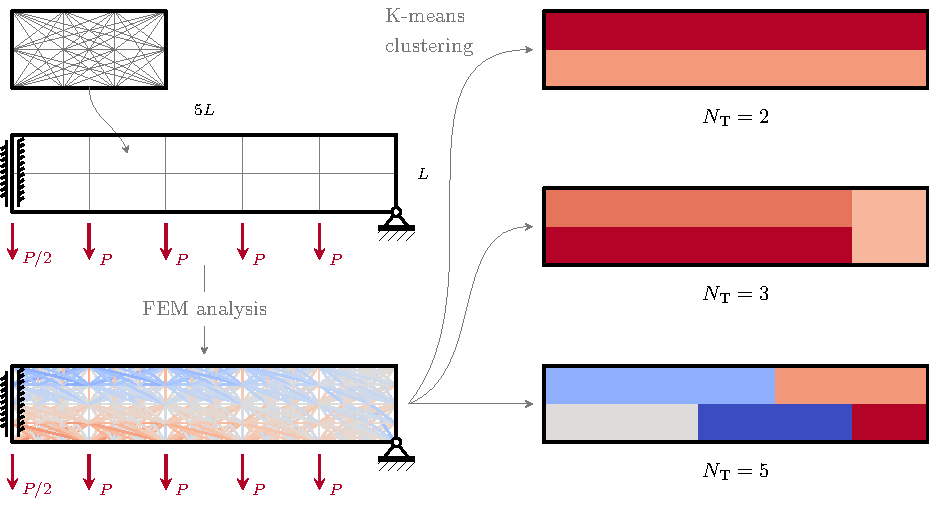
\includegraphics{figures/06_DMO/00_stress_clustering/stress_clustering.pdf}
    \caption{}
    \label{fig:06}
\end{figure*}

\begin{figure*}
    \centering
    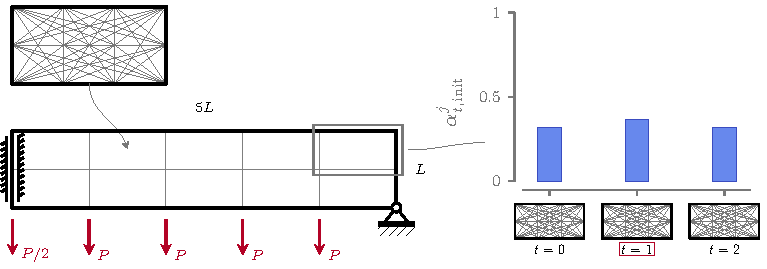
\includegraphics{figures/06_DMO/00_x0/x0.pdf}
    \caption{}
    \label{fig:06}
\end{figure*}

the initial layout of modules is assessed using a k meeans clustering technique with nt clusters. Given a set of observations (x1, x2, ..., xn), where each observation is a d-dimensional real vector, k-means clustering aims to partition the n observations into n sets. we define the observation as the vector containing the stress of the bars of unoptimized initial ground structure plus the stress state S For the j-th submodule we define the 

\begin{equation}
    S^j=\sum_{i=0}^{\bar{n}}|\sigma^j_i|
\end{equation}
This add permits to promote the clustering of not only submodules loaded in similar ways, but also on similar magnitude (and have so more voluminous and less voluminous modules).

\section{Numerical application}
IPOPT for the two steps

continuation scheme only on p (we use an interior point algo, we want to stay in the fesable region)
\subsection{Layout optimization of fixed modules}
\begin{marginfigure}
    \centering
    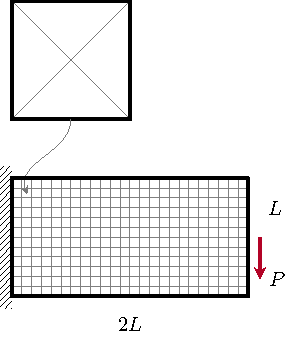
\includegraphics[width=\linewidth]{figures/06_DMO/00_cantilever_bcs/cant_mesh.pdf}
    \caption{Boundary conditions of the 2D cantilever beam divided in 24x12 subdomains. In the upper part of the image the ground structure of the module composed of $\bar{n}=6$ elements.}
    \label{fig:06_cant_BC_GS}
\end{marginfigure}
\begin{margintable}
    \small
    \centering
    \begin{tabular}{cc}
    \toprule
    \textbf{Parameter}        & \textbf{Value} \\ \midrule
    $L$              & 100     \\
    $\sigma_\text{c}, \sigma_\text{t}$ & $\pm 1$\\
    $P$              & 1   \\
    $a_\text{max}$              & 0.6   \\
    \bottomrule
    \end{tabular}
    \caption{Material data used for the 2D cantilever beam 2D.}
    \label{tab:06_modular_cant_data}
\end{margintable}
\begin{figure*}
    \subcaptionbox{}{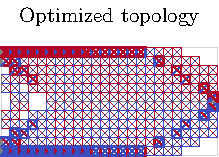
\includegraphics{figures/06_DMO/00_fixed_cells/top_00.pdf}}
    \hfill
    \subcaptionbox{}{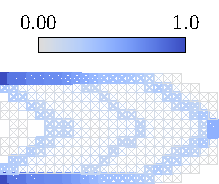
\includegraphics{figures/06_DMO/00_fixed_cells/weight_00.pdf}}
    \hfill
    \subcaptionbox{}{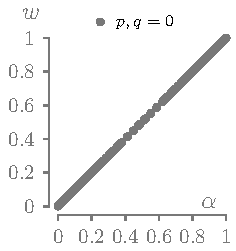
\includegraphics[height=3.5cm] {figures/06_DMO/00_fixed_cells/ramp_00.pdf}}
    \hfill
    \subcaptionbox{}{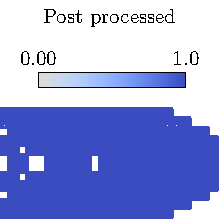
\includegraphics{figures/06_DMO/00_fixed_cells/weight_00_PP.pdf}}
    \bigskip
    \subcaptionbox{}{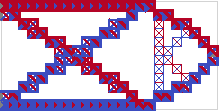
\includegraphics{figures/06_DMO/00_fixed_cells/top.pdf}}
    \hfill
    \subcaptionbox{}{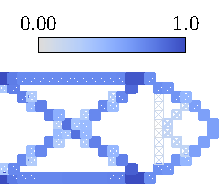
\includegraphics{figures/06_DMO/00_fixed_cells/weight.pdf}}
    \hfill
    \subcaptionbox{}{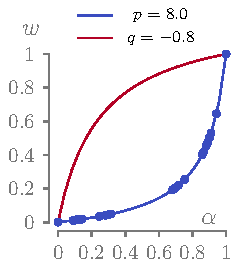
\includegraphics[height=3.5cm]{figures/06_DMO/00_fixed_cells/ramp.pdf}}
    \hfill
    \subcaptionbox{}{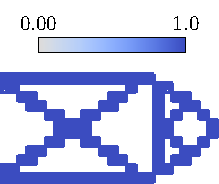
\includegraphics{figures/06_DMO/00_fixed_cells/weight_PP.pdf}}
    \caption{}
    \label{fig:06}
\end{figure*}

\begin{figure}
    \subcaptionbox{}{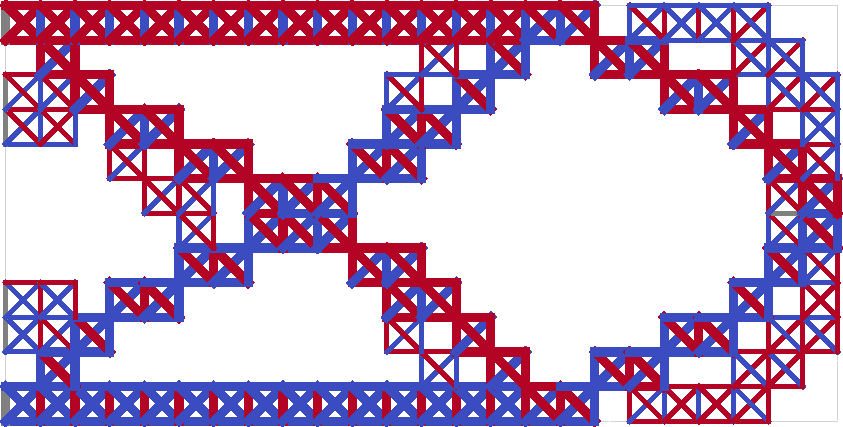
\includegraphics[width=0.45\linewidth]{figures/06_DMO/00_fixed_cells_multiple/fig1-Topology_area.pdf}}
    \hfill
    \subcaptionbox{}{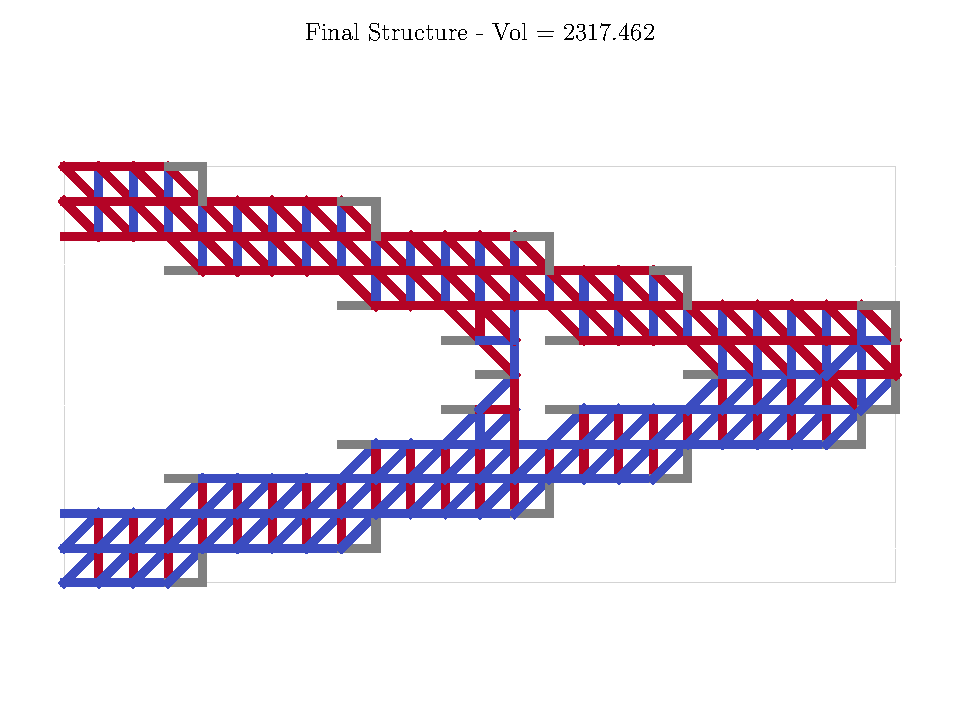
\includegraphics[width=0.45\linewidth]{figures/06_DMO/00_fixed_cells_multiple/fig1-Topology_topol.pdf}}
    \hfill
    \bigskip
    \subcaptionbox{}{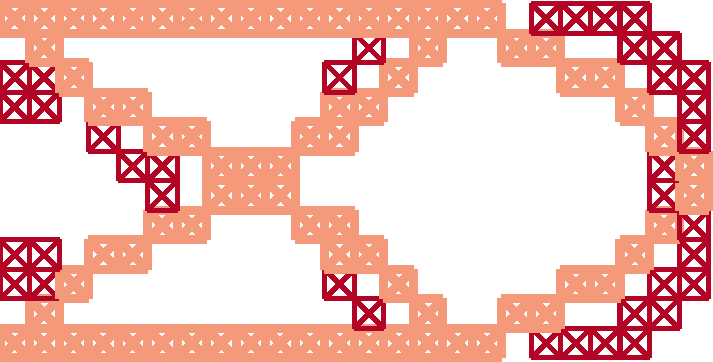
\includegraphics[width=0.45\linewidth]{figures/06_DMO/00_fixed_cells_multiple/fig12-Module_withType_area.pdf}}
    \hfill
    \subcaptionbox{}{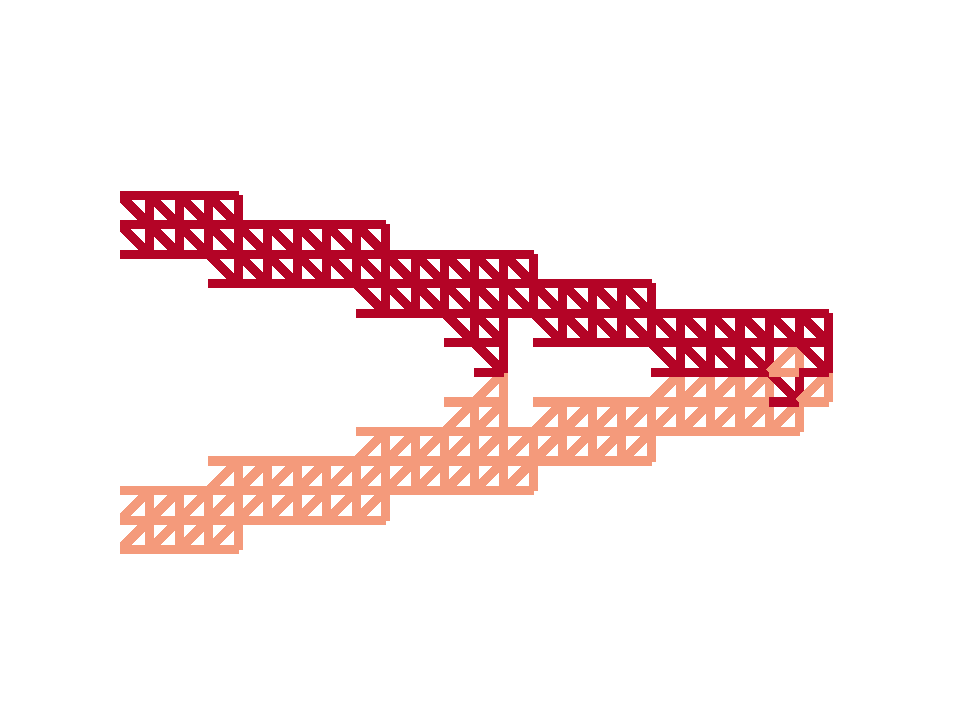
\includegraphics[width=0.45\linewidth]{figures/06_DMO/00_fixed_cells_multiple/fig12-Module_withType_topol.pdf}}
    \caption{}
    \label{fig:06}
\end{figure}
\subsection{Modules and layout optimization}
\begin{figure}
    \hspace*{\fill}
    \subcaptionbox{}{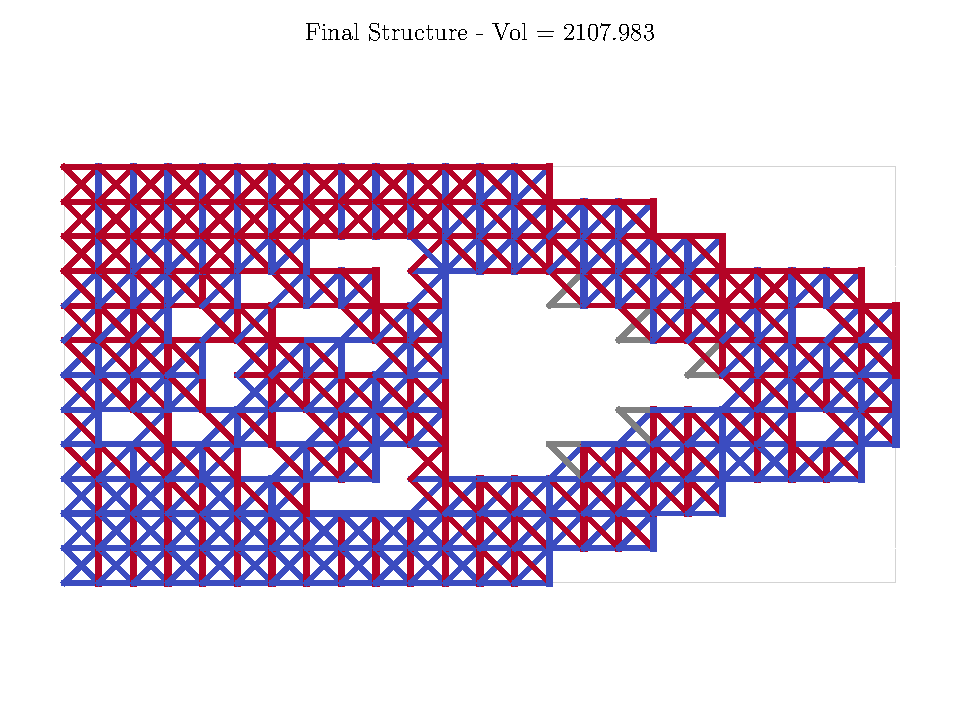
\includegraphics[width=0.45\linewidth]{figures/06_DMO/00_optimized_module/fig1-Topology.pdf}}
    \hfill
    \subcaptionbox{}{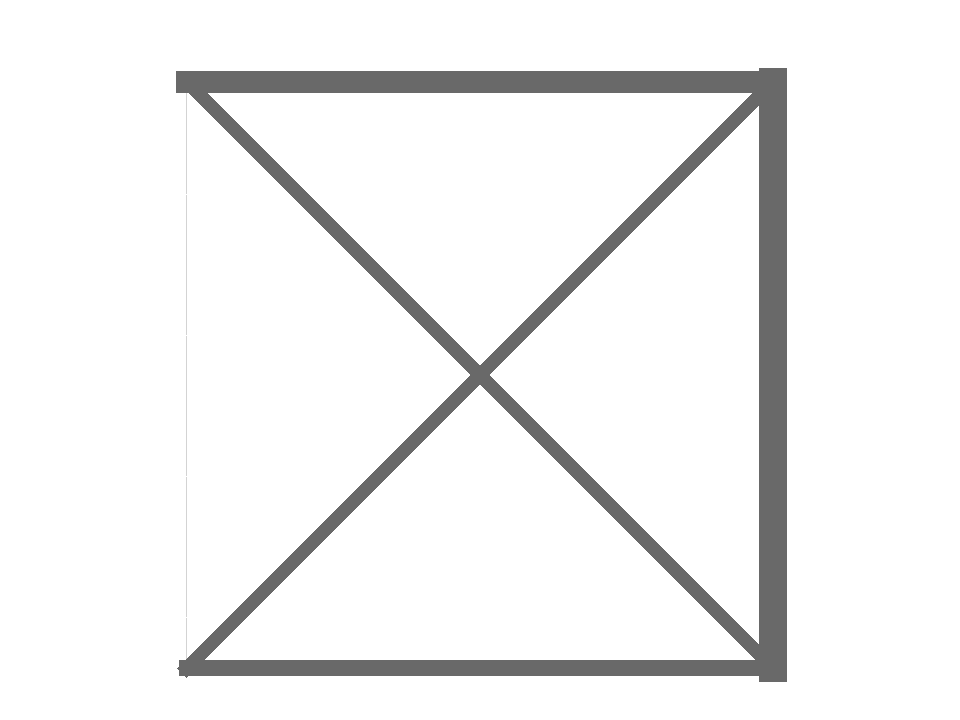
\includegraphics[width=0.3\linewidth]{figures/06_DMO/00_optimized_module/fig8-Module_Topology_001.pdf}}
    \hspace*{\fill}
    \caption{}
    \label{fig:06}
\end{figure}
\todo{tables with volume and phi and psi for different NT}

\begin{figure}
    \centering
    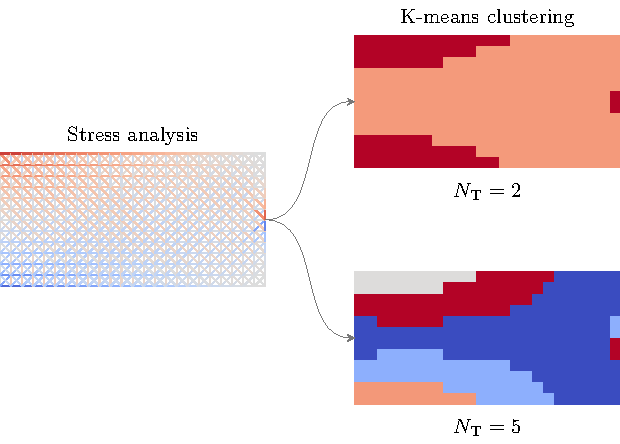
\includegraphics{figures/06_DMO/00_optimized_modules/kmeans.pdf}
    \caption{}
    \label{fig:06}
\end{figure}

\begin{figure*}
    \subcaptionbox{}{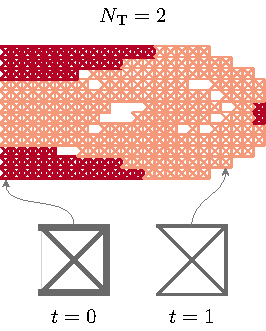
\includegraphics[width=0.3\linewidth]{figures/06_DMO/00_optimized_modules/nt2.pdf}}
    \hfill
    \subcaptionbox{}{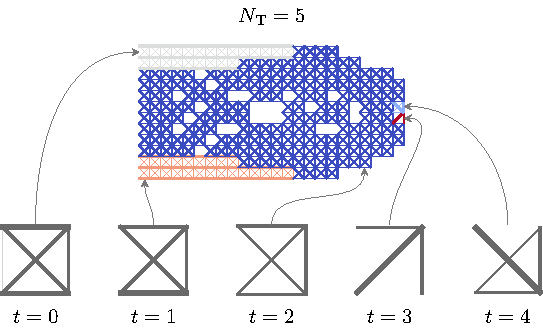
\includegraphics[width=0.6\linewidth]{figures/06_DMO/00_optimized_modules/nt5.pdf}}
    \caption{}
    \label{fig:06}
\end{figure*}

\subsection{A benchmark case study: a simply supported modular bridge}

\todo{difference with tugilimana, we take into account the buckling whensolving the first subproblem of module layout, we can have an empty subdomain andwe use a gradeint descent algo}

\begin{figure}
    \centering
    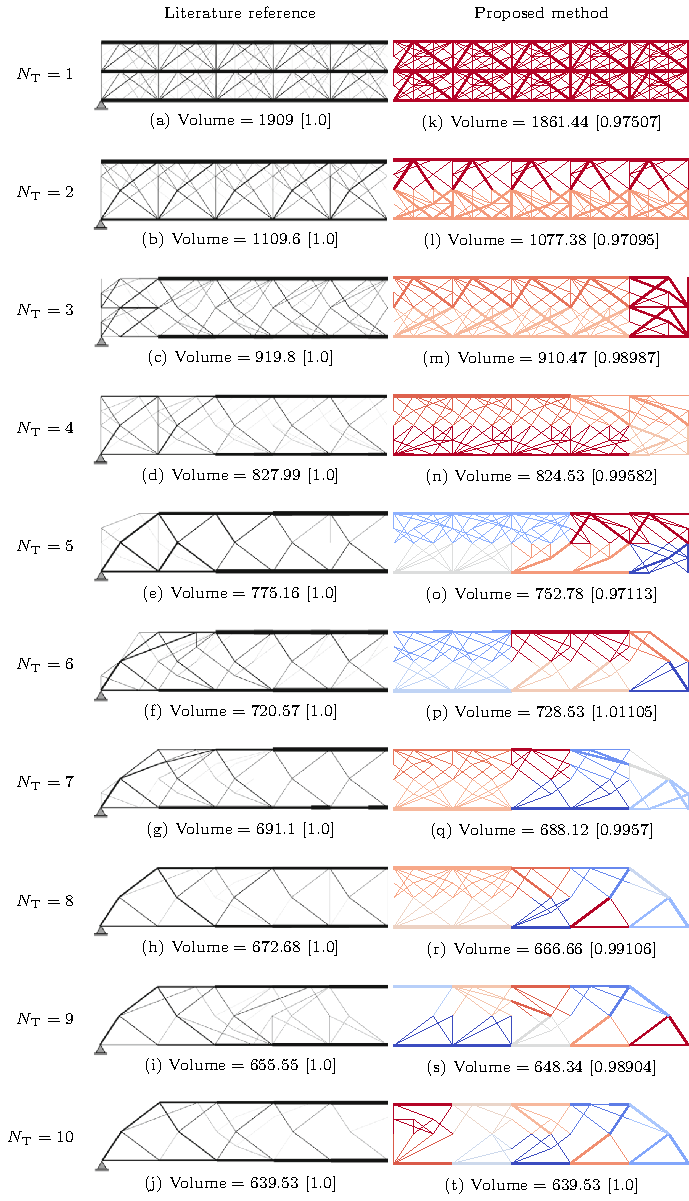
\includegraphics{figures/06_DMO/00_tug_bench/bench.pdf}
    \caption{}
    \label{fig:06}
\end{figure}

\begin{figure}
    \centering
    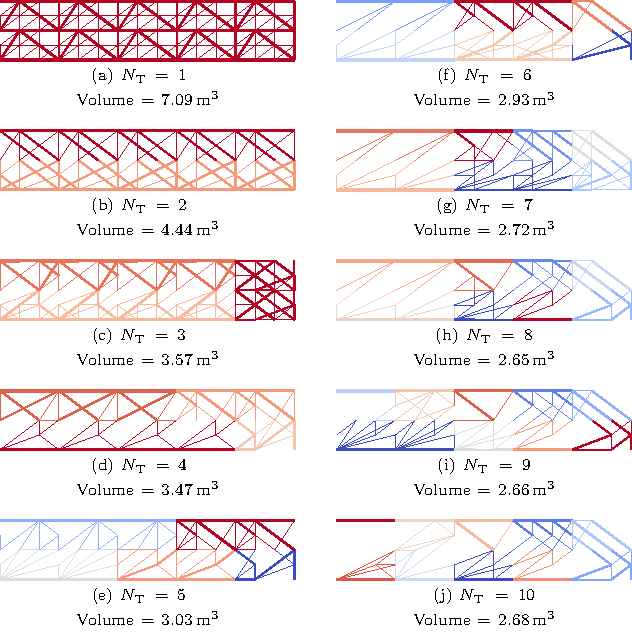
\includegraphics{figures/06_DMO/00_tug_bench_buck/buck.pdf}
    \caption{}
    \label{fig:06}
\end{figure}

\begin{figure*}
    \centering
    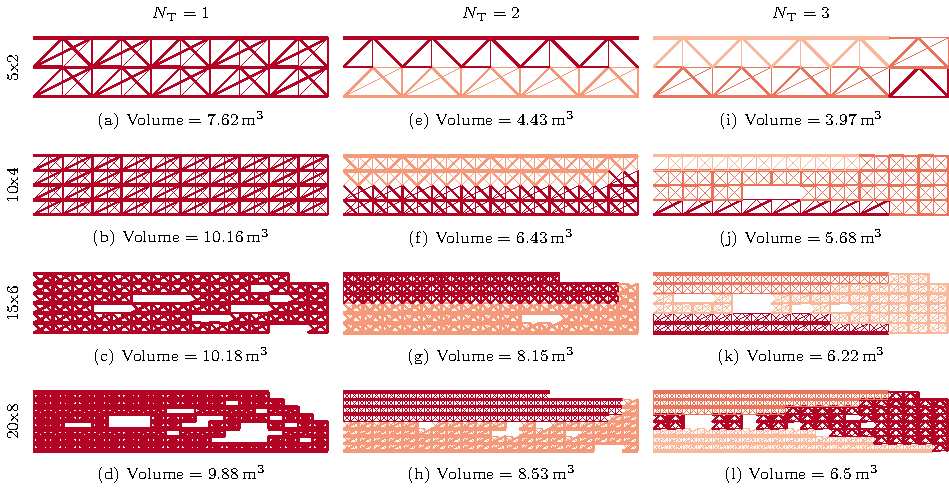
\includegraphics{figures/06_DMO/00_tug_bench_size/size.pdf}
    \caption{}
    \label{fig:06}
\end{figure*}
principalmente due motivi, cambia il metodo di rottura, non piu buckling e poi ho i vuoti

\subsection{Simply supported 3D beam}
\begin{margintable}
    \small
    \centering
    \begin{tabular}{cc}
    \toprule
    \textbf{Parameter}        & \textbf{Value} \\ \midrule
    $E$              & \qty{2.7}{GPa}     \\
    $\nu$            & 0.3   \\
    $\sigma_\text{c}, \sigma_\text{t}$ & $\pm $\qty{55}{MPa} \\
    $\rho$              & \qty{1.14}{\gram\per\cubic\centi\metre}   \\
    $P$              & \qty{100}{N}   \\
    \bottomrule
    \end{tabular}
    \caption{Material data used for the simply supported 3D beam optimization.}
    \label{tab:06_3D_supp_mat}
\end{margintable}

\begin{figure*}
    \hspace*{\fill}
    \subcaptionbox{}{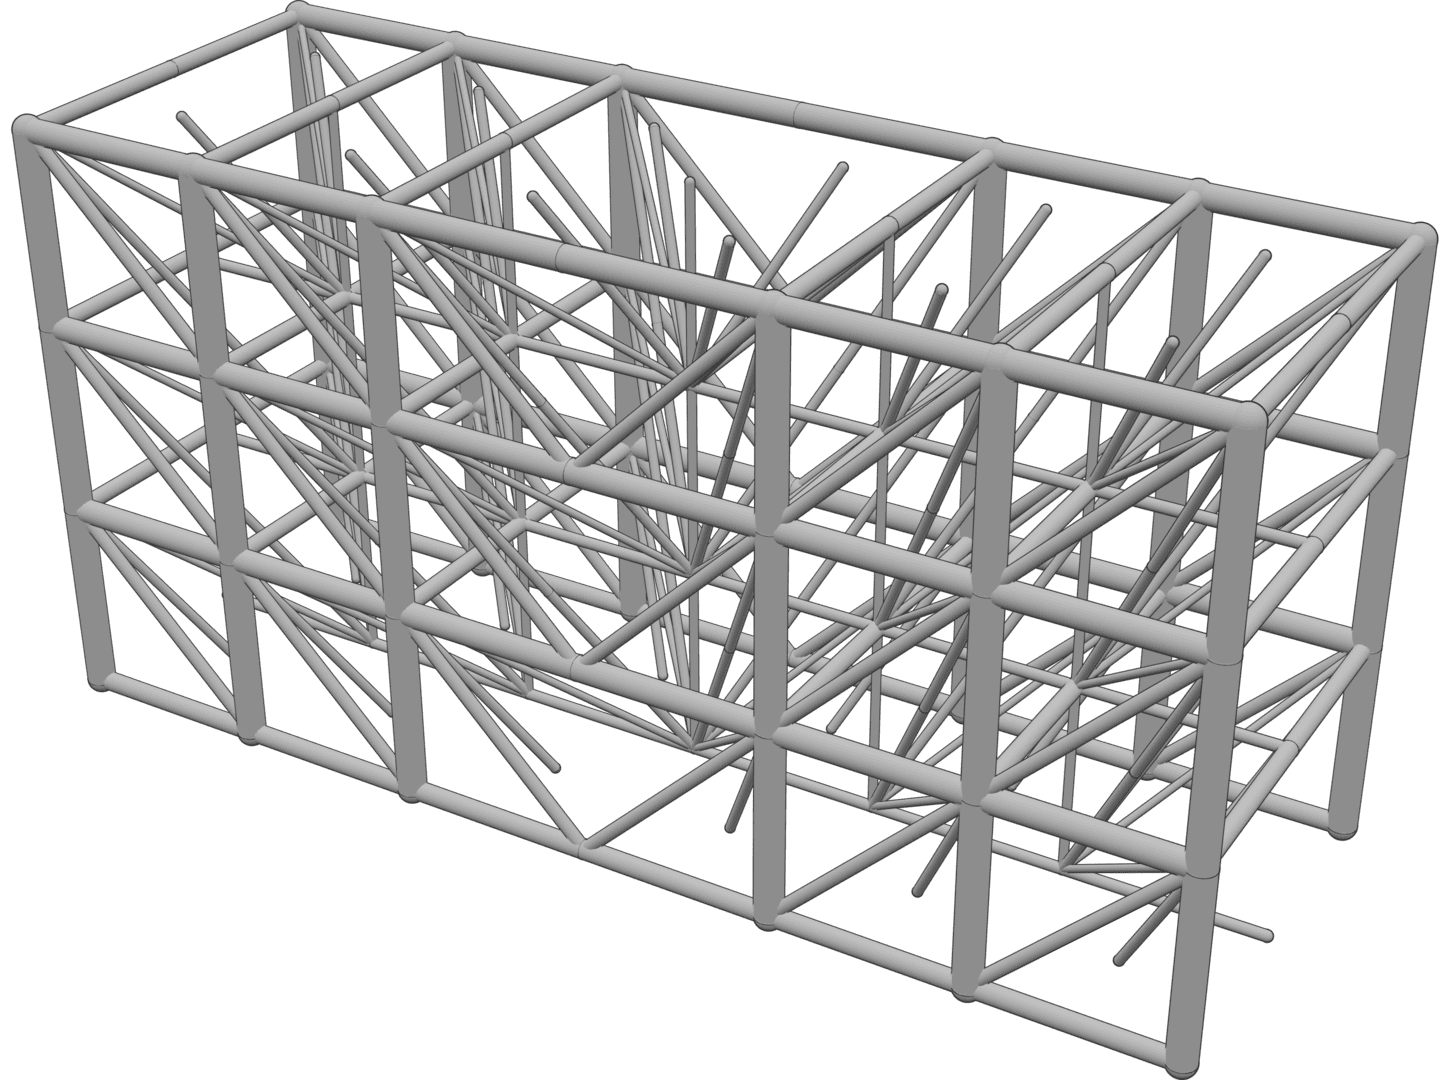
\includegraphics[width=0.30\linewidth]{figures/06_DMO/00_print_topology/1_04_Topology_NLP_iso.png}}
    \hfill
    \subcaptionbox{}{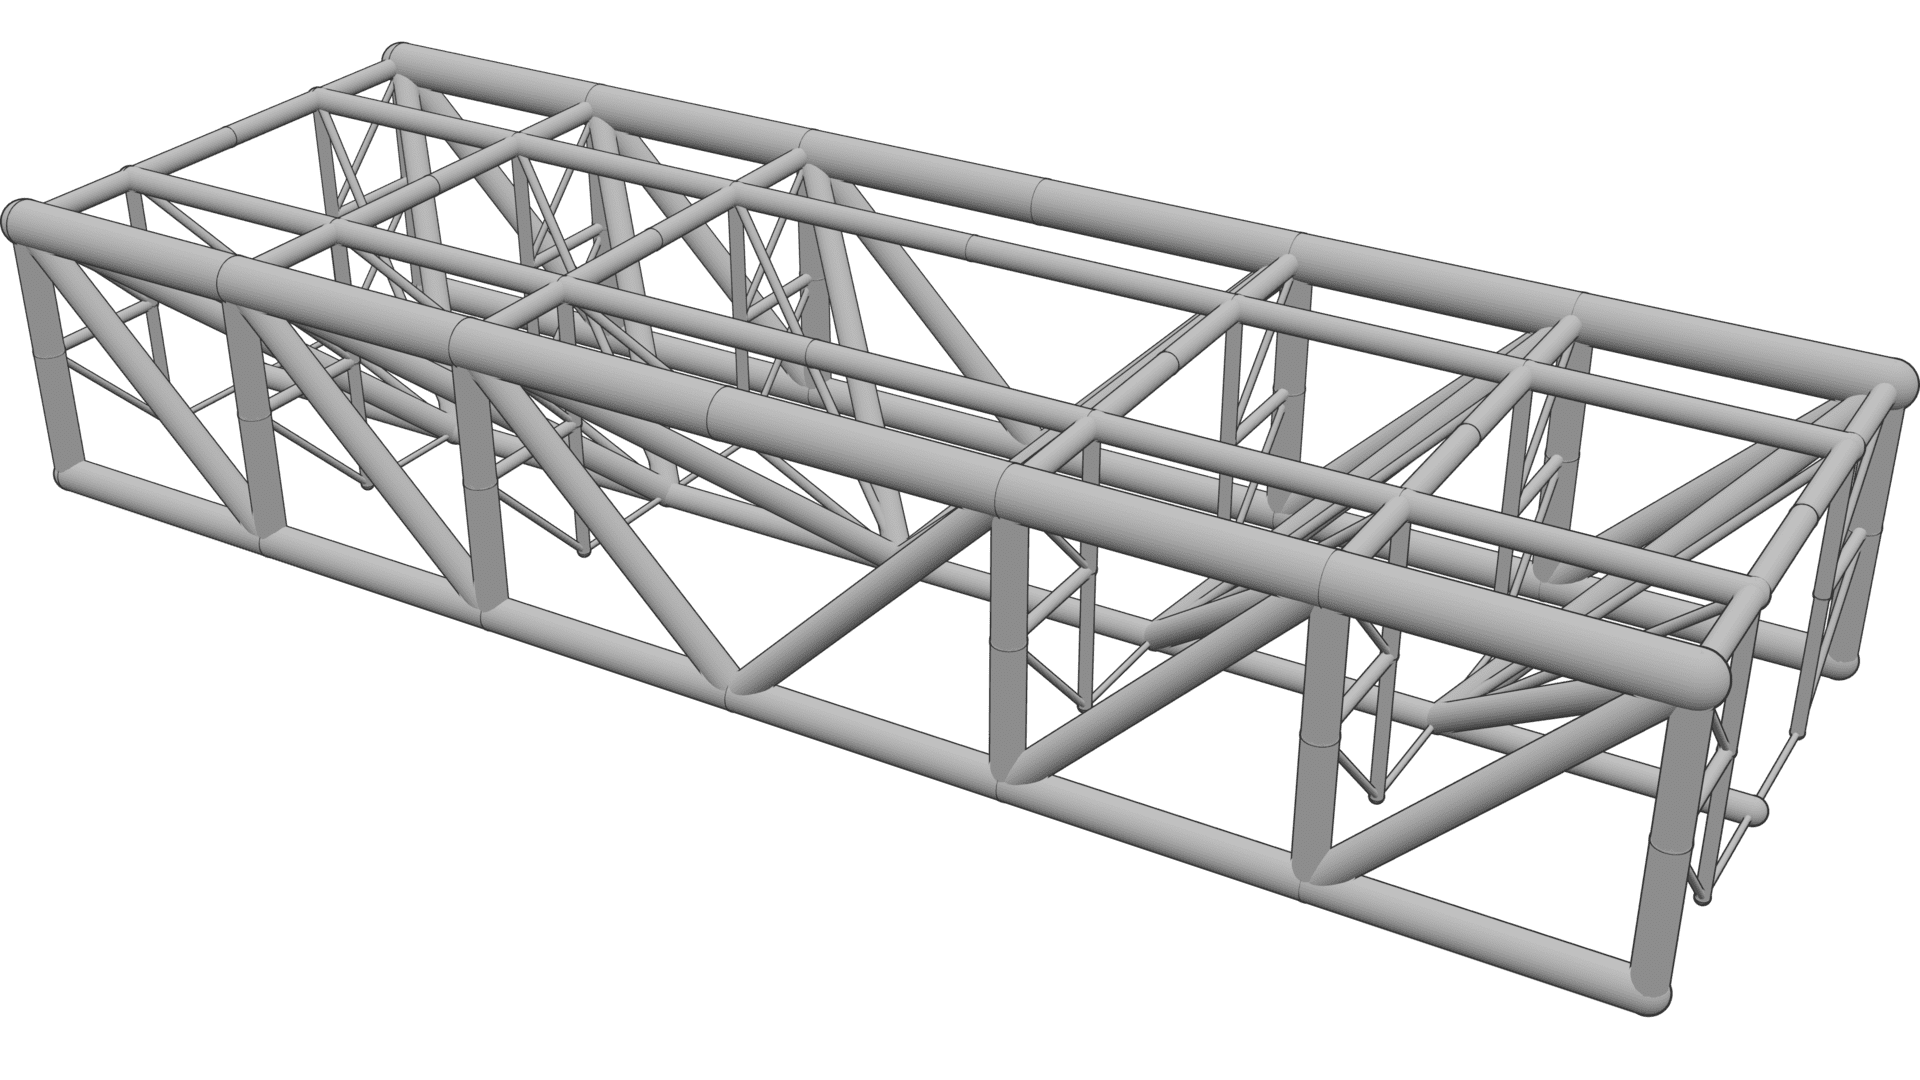
\includegraphics[width=0.30\linewidth]{figures/06_DMO/00_print_topology/2_04_Topology_NLP_iso.png}}
    \hfill
    \subcaptionbox{}{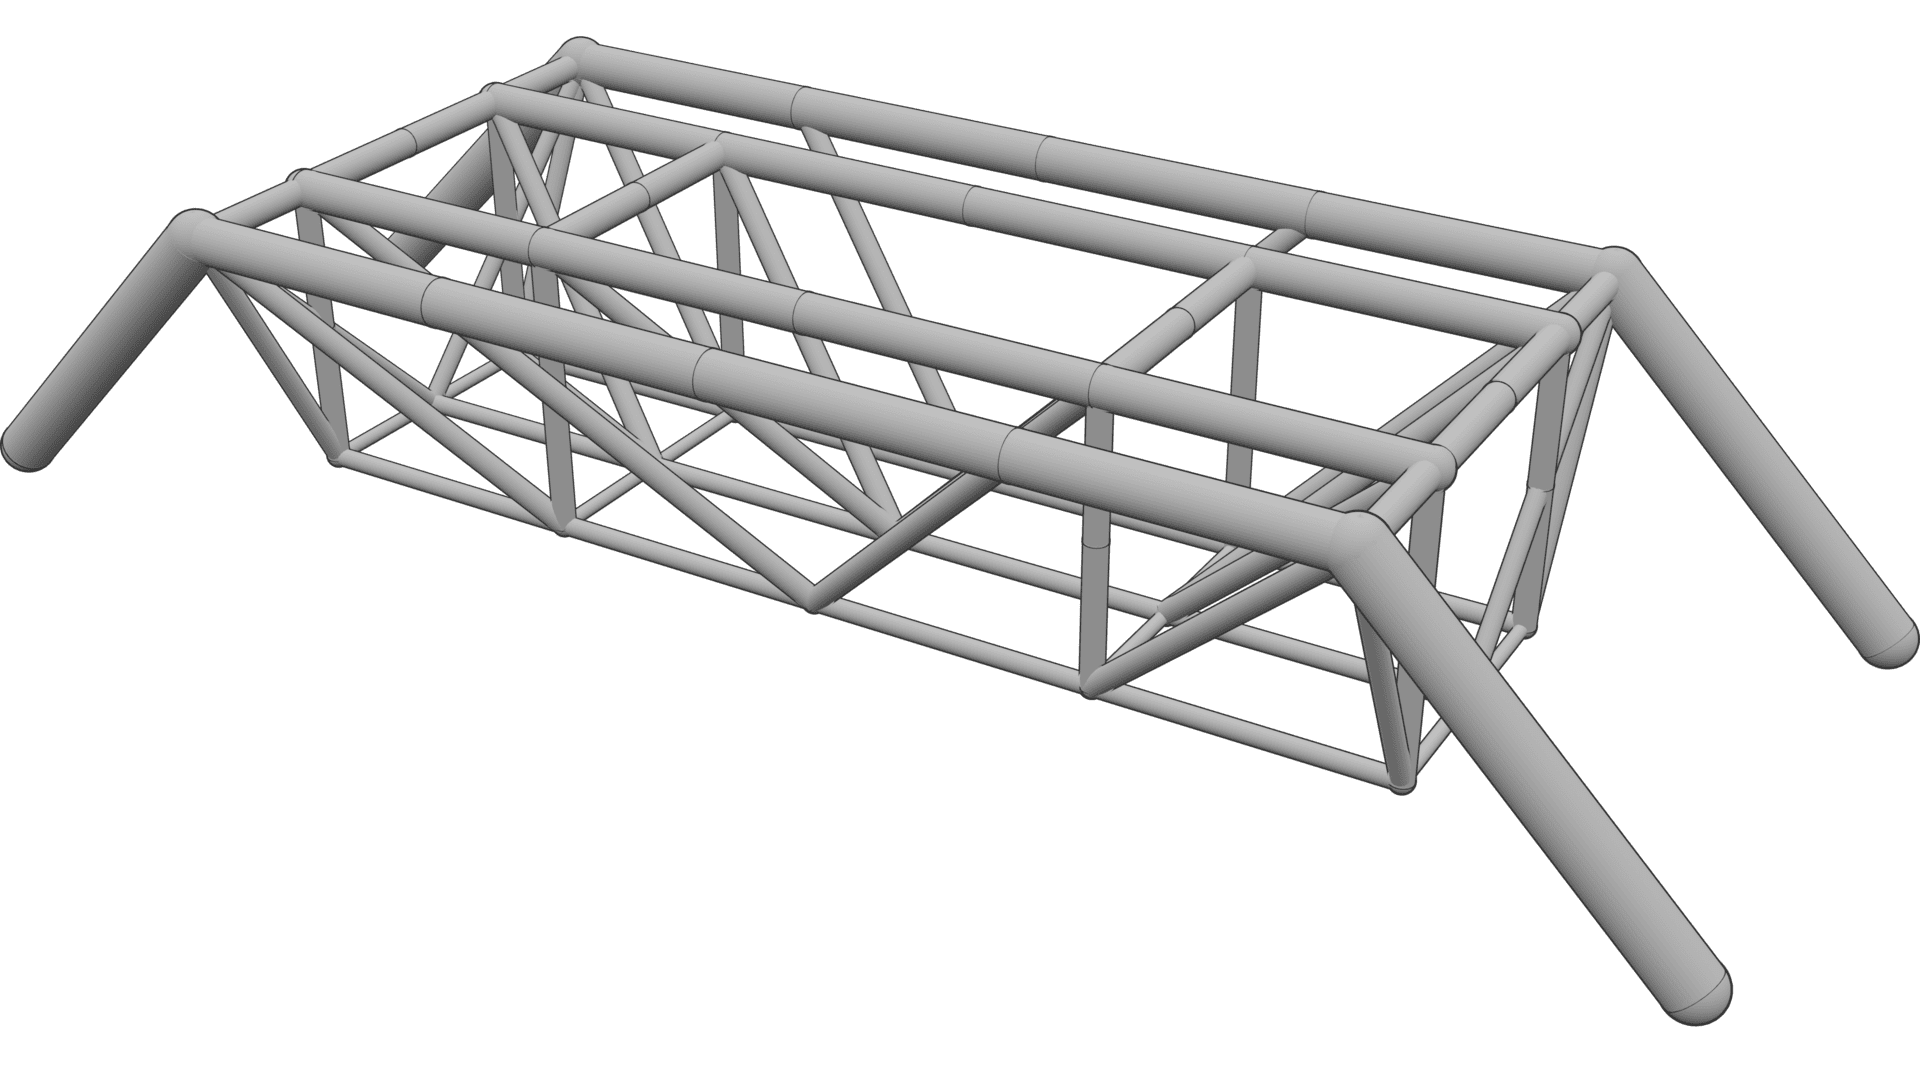
\includegraphics[width=0.30\linewidth]{figures/06_DMO/00_print_topology/3_04_Topology_NLP_iso.png}}
    \hspace*{\fill}
    \bigskip
    \hspace*{\fill}
    \subcaptionbox{}{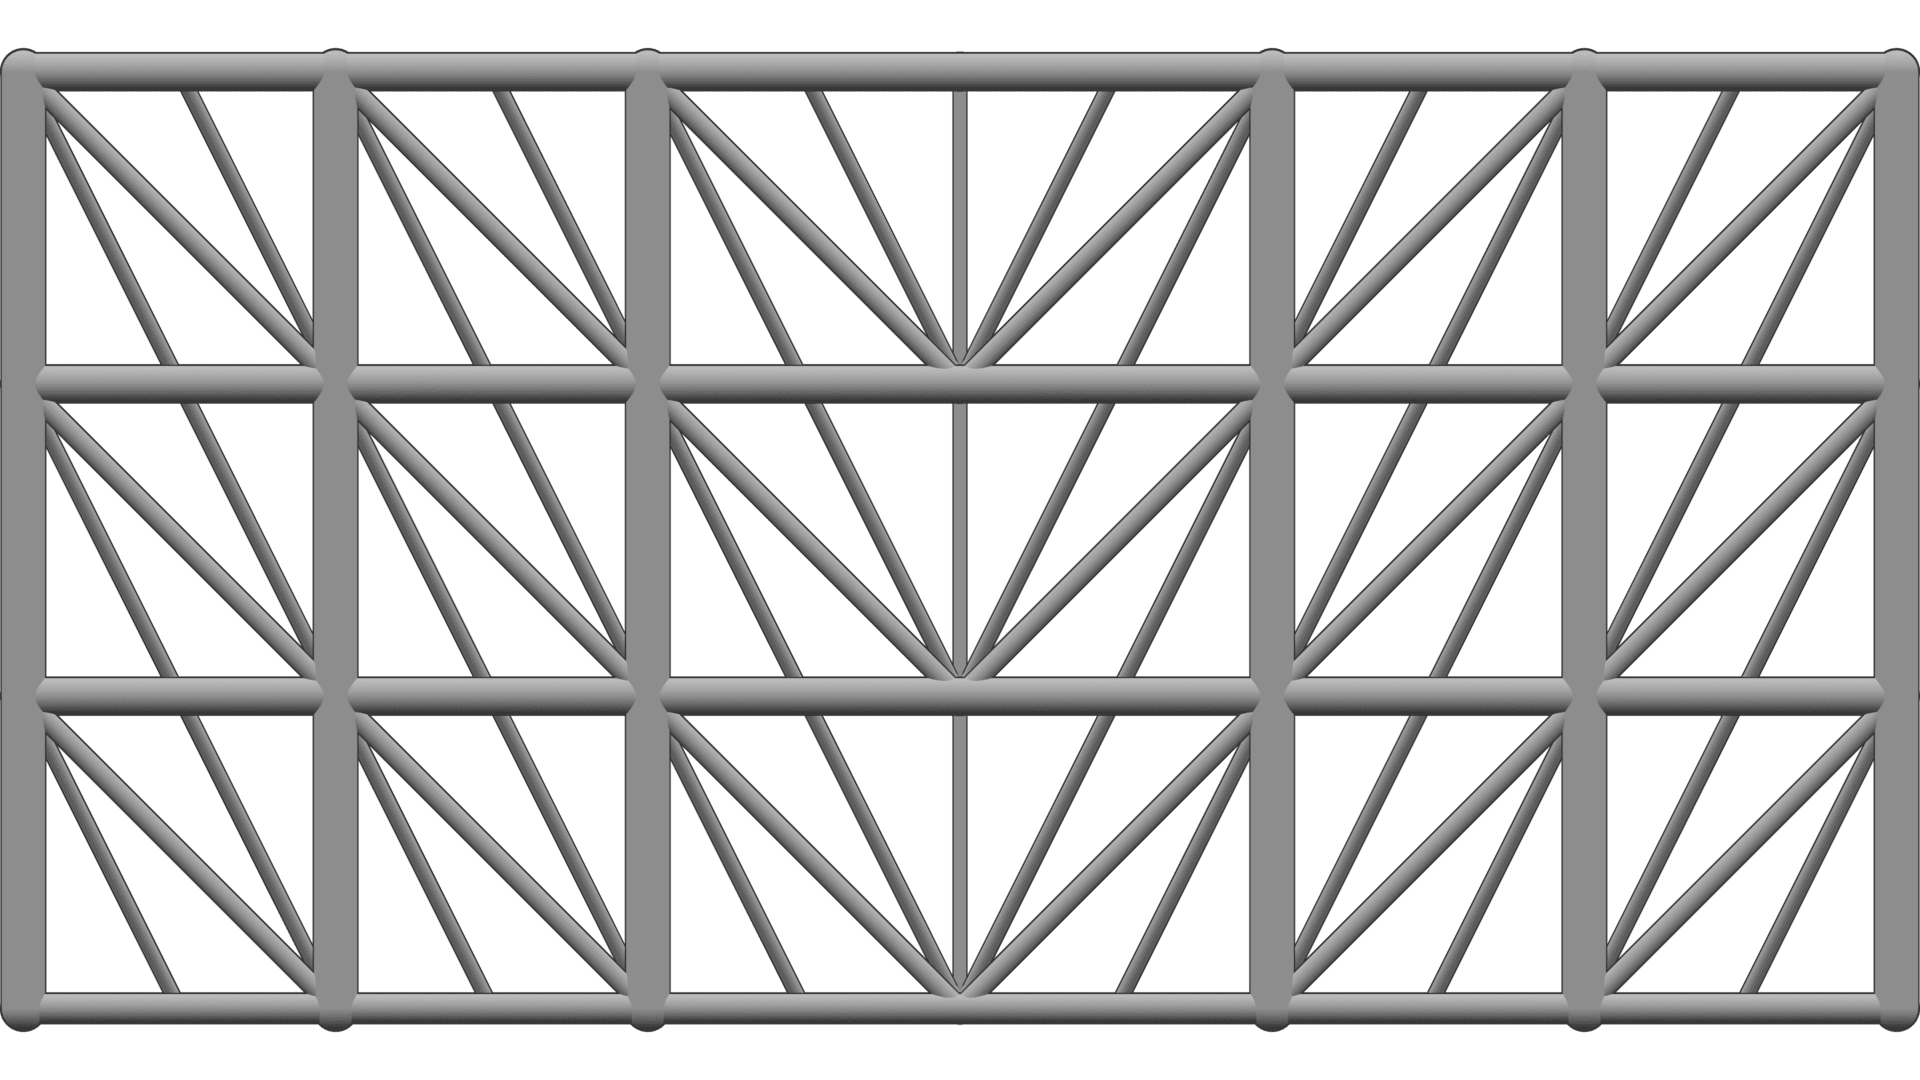
\includegraphics[width=0.30\linewidth]{figures/06_DMO/00_print_topology/1_04_Topology_NLP_XZ.png}}
    \hfill
    \subcaptionbox{}{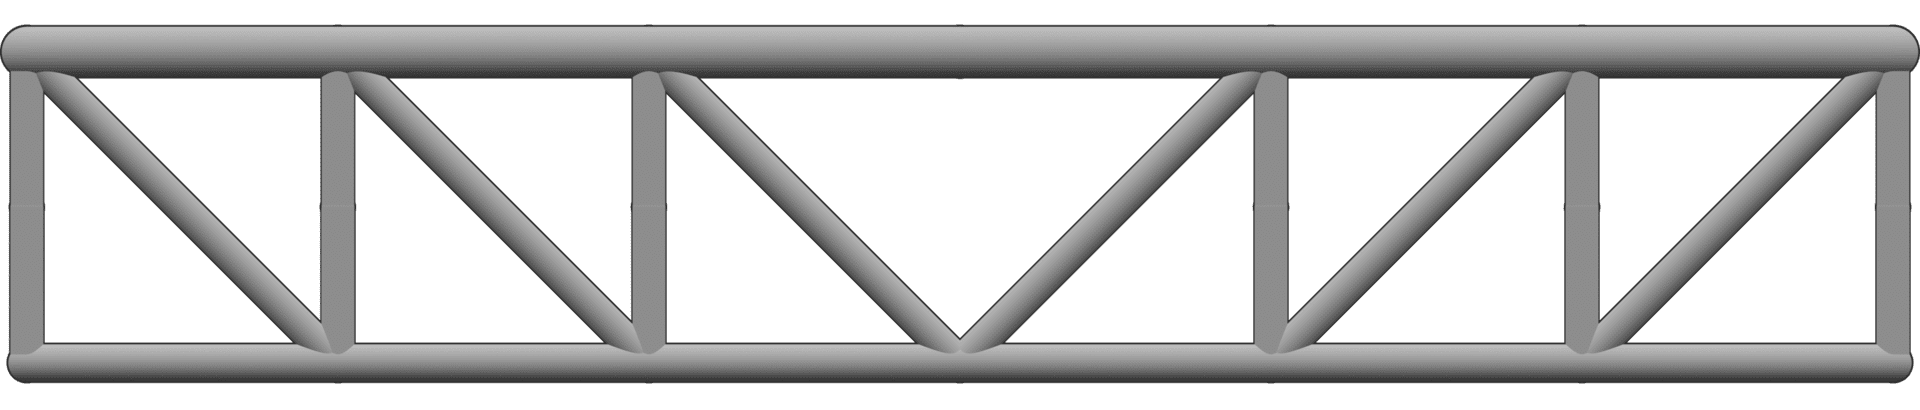
\includegraphics[width=0.30\linewidth]{figures/06_DMO/00_print_topology/2_04_Topology_NLP_XZ.png}}
    \hfill
    \subcaptionbox{}{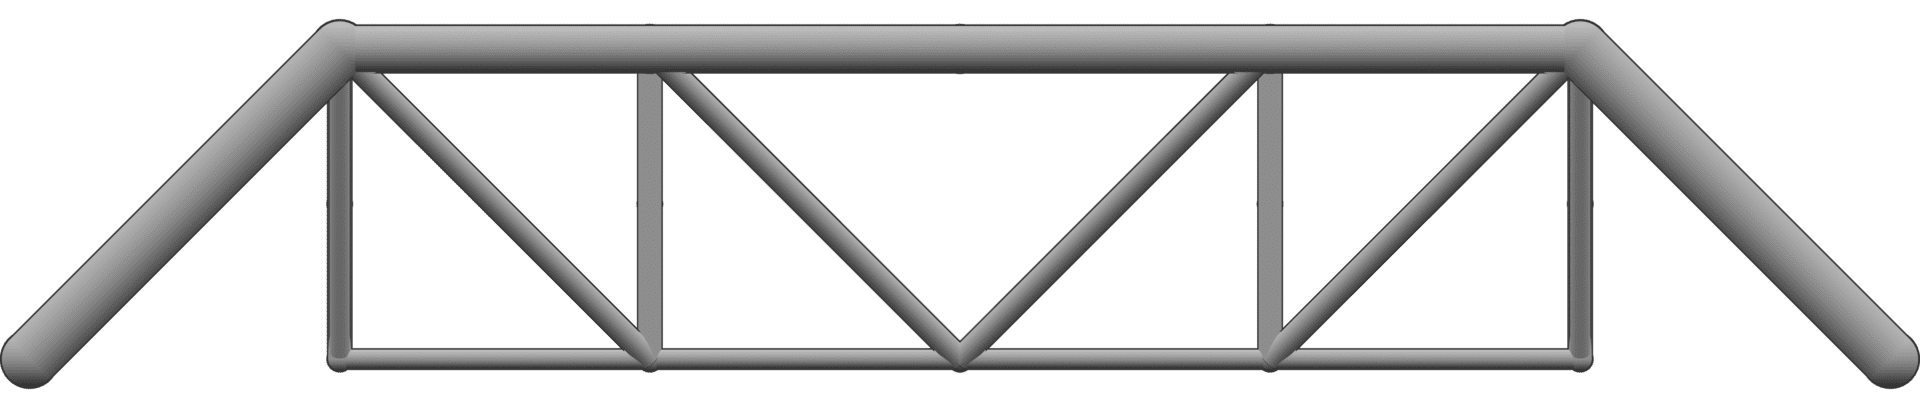
\includegraphics[width=0.30\linewidth]{figures/06_DMO/00_print_topology/3_04_Topology_NLP_XZ.png}}
    \hspace*{\fill}
    \caption{}
    \label{fig:06}
\end{figure*}

\begin{table}
    \centering
    \small
    \begin{tabular}{lx{1.8cm}x{1.8cm}x{1.8cm}x{1.8cm}}
        \toprule
    $N_\text{T}$ & --     & 1     &  2    &  3  \\ \midrule
    $N_\text{sub}$           &    1  &   36   &   36   &   36     \\
    $N_\text{opt}\;(N_\text{el})$  &  20 (1984) &  360 (12636)   &  204 (12636)   &  104 (12636)        \\
    $V$ [\unit{cm^3}] & 9.907 &  27.958 &   15.548  & 10.178    \\
    $V$ [\unit{\percent}] & 1.761 & 4.970&2.764 & 1.809    \\
    $\bar{\rho}$ [\unit{kg/m^3}] & 80.31 &226.65 &126.05 &82.51 \\
    C [\unit{J}]      &  3.71  &  5.20   &  6.21  & 4.141  \\
    $a_\text{max}$ [\unit{mm^2}]      & 37.61& 9.40  & 12.81  &   15.81     \\
    $\varphi$   &\qty{100.00}{\percent}&\qty{21.11}{\percent}&\qty{39.21}{\percent}&\qty{80.77}{\percent}  \\
    $\psi$& 1.00   &  0.47 &  0.66   & 0.87        \\
    t        & \hms{0;0;4}  &  \hms{0;1;18} & \hms{0;0;42} & \hms{0;10;22}   \\ \bottomrule
    \end{tabular}
    \caption{}
    \label{tab:06}
    \end{table}

\section{Conclusion}